\documentclass{article}\usepackage[]{graphicx}\usepackage[]{color}
%% maxwidth is the original width if it is less than linewidth
%% otherwise use linewidth (to make sure the graphics do not exceed the margin)
\makeatletter
\def\maxwidth{ %
  \ifdim\Gin@nat@width>\linewidth
    \linewidth
  \else
    \Gin@nat@width
  \fi
}
\makeatother

\definecolor{fgcolor}{rgb}{0.345, 0.345, 0.345}
\newcommand{\hlnum}[1]{\textcolor[rgb]{0.686,0.059,0.569}{#1}}%
\newcommand{\hlstr}[1]{\textcolor[rgb]{0.192,0.494,0.8}{#1}}%
\newcommand{\hlcom}[1]{\textcolor[rgb]{0.678,0.584,0.686}{\textit{#1}}}%
\newcommand{\hlopt}[1]{\textcolor[rgb]{0,0,0}{#1}}%
\newcommand{\hlstd}[1]{\textcolor[rgb]{0.345,0.345,0.345}{#1}}%
\newcommand{\hlkwa}[1]{\textcolor[rgb]{0.161,0.373,0.58}{\textbf{#1}}}%
\newcommand{\hlkwb}[1]{\textcolor[rgb]{0.69,0.353,0.396}{#1}}%
\newcommand{\hlkwc}[1]{\textcolor[rgb]{0.333,0.667,0.333}{#1}}%
\newcommand{\hlkwd}[1]{\textcolor[rgb]{0.737,0.353,0.396}{\textbf{#1}}}%
\let\hlipl\hlkwb

\usepackage{framed}
\makeatletter
\newenvironment{kframe}{%
 \def\at@end@of@kframe{}%
 \ifinner\ifhmode%
  \def\at@end@of@kframe{\end{minipage}}%
  \begin{minipage}{\columnwidth}%
 \fi\fi%
 \def\FrameCommand##1{\hskip\@totalleftmargin \hskip-\fboxsep
 \colorbox{shadecolor}{##1}\hskip-\fboxsep
     % There is no \\@totalrightmargin, so:
     \hskip-\linewidth \hskip-\@totalleftmargin \hskip\columnwidth}%
 \MakeFramed {\advance\hsize-\width
   \@totalleftmargin\z@ \linewidth\hsize
   \@setminipage}}%
 {\par\unskip\endMakeFramed%
 \at@end@of@kframe}
\makeatother

\definecolor{shadecolor}{rgb}{.97, .97, .97}
\definecolor{messagecolor}{rgb}{0, 0, 0}
\definecolor{warningcolor}{rgb}{1, 0, 1}
\definecolor{errorcolor}{rgb}{1, 0, 0}
\newenvironment{knitrout}{}{} % an empty environment to be redefined in TeX

\usepackage{alltt}
\title{Descriptive Analyses} 
\author{Francois Rerolle}
\date{\today}

%List if latex packages you'll need
\usepackage{float}
\usepackage{mathtools}
\usepackage{graphicx}
\graphicspath{{/Users/francoisrerolle/Desktop/UCSF/Dissertation/Paper-1-Geospatial-Analysis-Forest-Incidence/Analyses/figure/}}

%set the margins of the document
\usepackage[]{geometry}

%End the preamble and begin the document
\IfFileExists{upquote.sty}{\usepackage{upquote}}{}
\begin{document}
\maketitle
 

\noindent \textit{Report of some descriptive statistics on the final cleaned dataset (A3 + environmental covariates).}

%%%%%%%%%%%%%%%%%%%%%%%%%%%%%%%%%%%%%%%%%
% Start by a description of the dataset %
%%%%%%%%%%%%%%%%%%%%%%%%%%%%%%%%%%%%%%%%%

\section{Description of dataset}
\subsection{What, where and when}
In 2017, we collected all A3 forms available in 4 districts of the southern province of Champasak in Laos: Moonlapamok, Pathoomphone, Sanasomboon and Sukhuma. A3 forms record all suspected malaria cases passively detected that got tested for malaria by RDT and/or microscopy.\\

\noindent A total of \(64503\) A3 forms were collected. Individuals reported coming from \(507\) villages (\(4.2\) $\%$ missing) in \(8\) districts (\(0\) $\%$ missing). Most individuals lived in districts where A3 form was collected but some lived in other districts:\\

\begin{knitrout}
\definecolor{shadecolor}{rgb}{0.969, 0.969, 0.969}\color{fgcolor}\begin{kframe}
\begin{verbatim}
## 
##    Champasak        Khong  Moonlapamok     Paksxong Pathoomphone 
##          958          578        15741            2        24316 
##   Phongthong  Sanasomboon      Sukhuma         <NA> 
##            3        14158         8747            0
\end{verbatim}
\end{kframe}
\end{knitrout}

\noindent Figure \ref{fig:Histogram_Date} shows a time distribution of A3 forms ranging from \(2013-09-25\) to \(2016-12-29\), pretty constant over a 3 year period from October 2013 to October 2016. Figure \ref{fig:Histogram_Date_District} shows that this true across the 4 districts of data collection.

\begin{figure}
\begin{center}

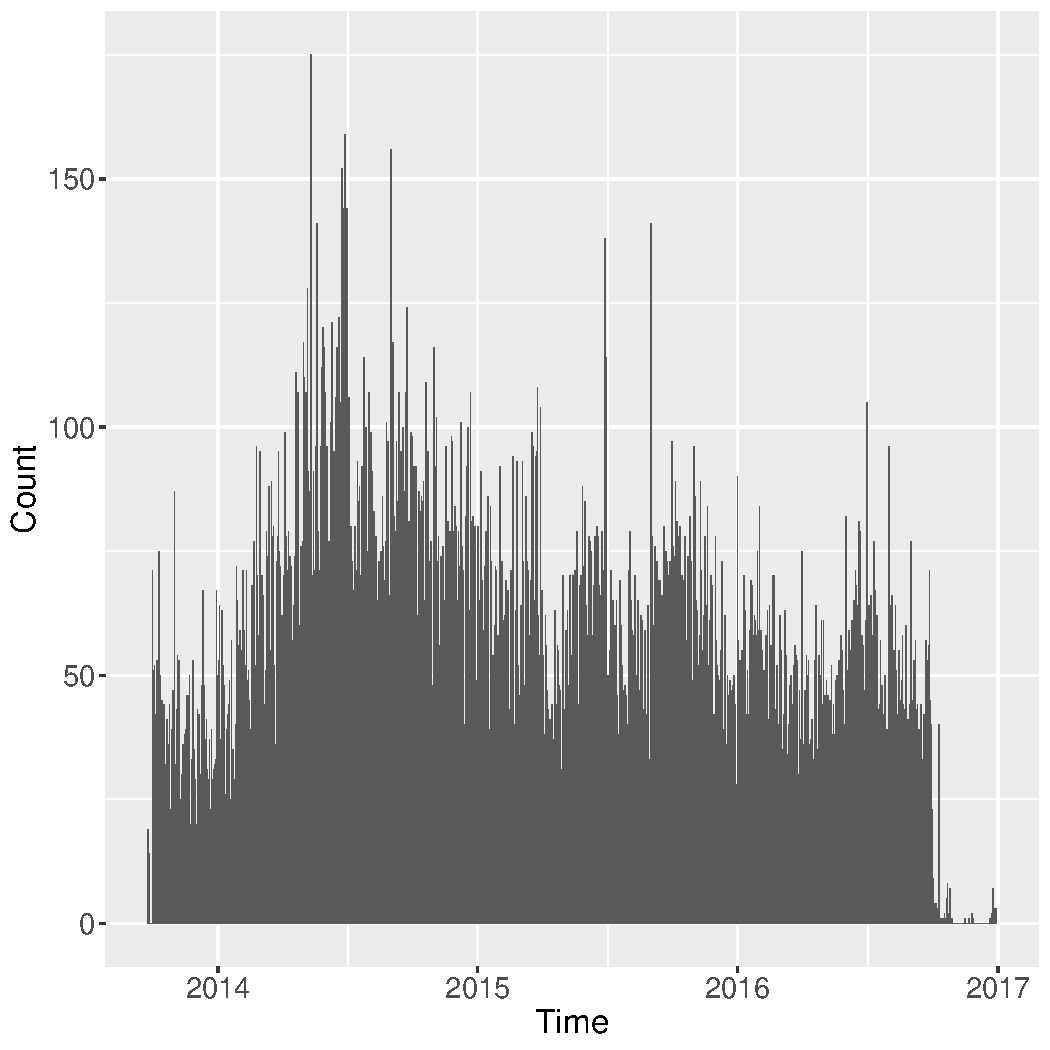
\includegraphics[width=0.5\textwidth]{fig1-1}
\end{center}
\caption{Histogram of A3 data collection times.}
\label{fig:Histogram_Date}
\end{figure}

\begin{figure}
\begin{center}

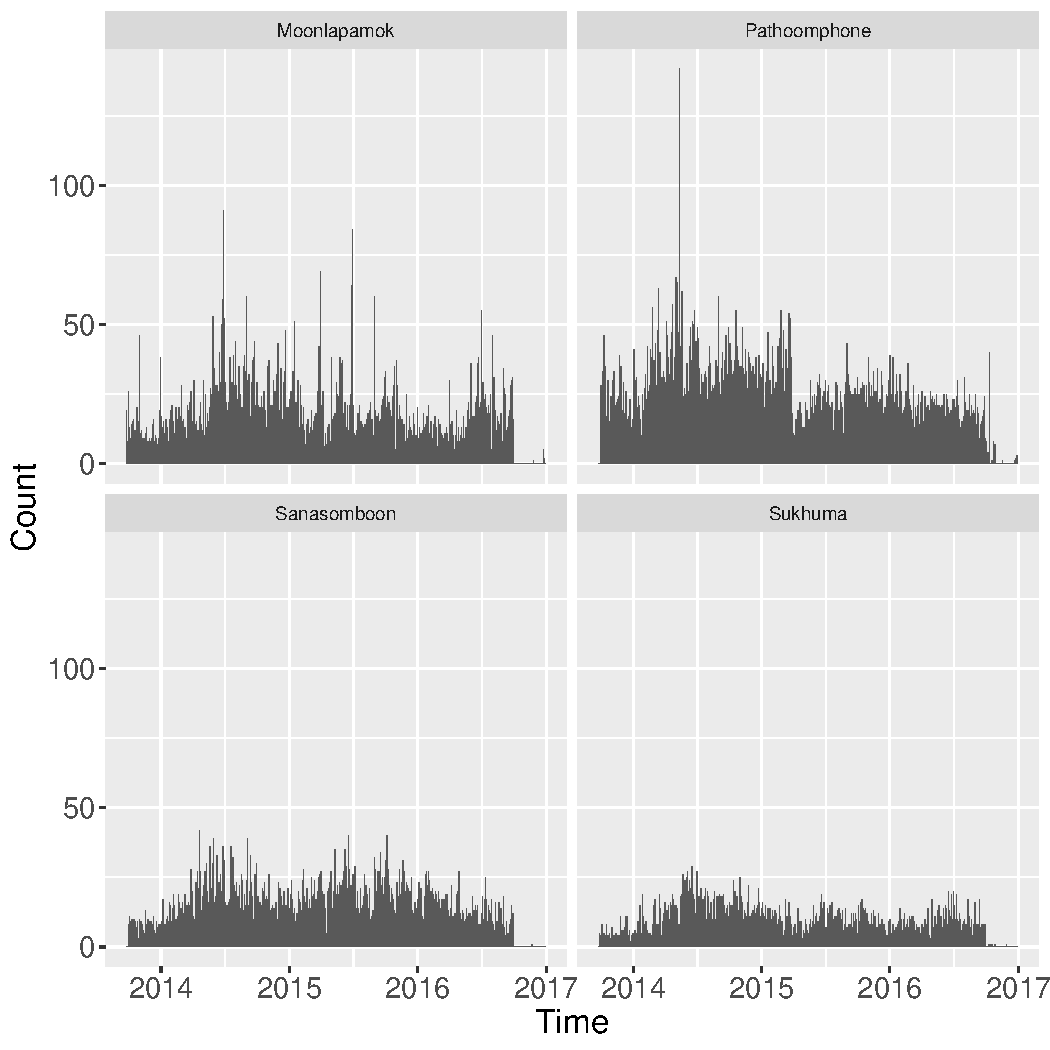
\includegraphics[width=0.5\textwidth]{fig2-1}
\end{center}
\caption{Histogram of A3 data collection times per district.}
\label{fig:Histogram_Date_District}
\end{figure}

\subsection{Description of variables}
There are two types of variables available in this dataset:
\begin{itemize}
\item Variables that were collected in the A3 form: date, district, village, age, gender, occupation, RDT result, microscopy result and treatment taken.
\item Environmental covariates that were extracted from raster layers via GPS coordinates of villages (matched via offical list of villages in Champasak): altitude, temperature, precipitation, population, percent High-Biomass Vegetation (HBV) in 1km and percent High-Biomass Vegetation (HBV) in 10km.
\end{itemize}

%%%%%%%%%%%%%%%%%%%%%%%%%%
% Descriptive Statistics %
%%%%%%%%%%%%%%%%%%%%%%%%%%

\section{Descriptive statistics}
\subsection{Basic description}


\begin{table}[htp]
\begin{center}
\begin{tabular}{lp{11cm}c}
Variable & Description & Missing \\ \hline
&& \\
Date & Date of the A3 interview, over 3 years from October 2013 to 2016 & \(0.3\) $\%$ \\
&& \\
District & Reported district where living. \(8\) different districts of Champasak Province. \(97.6\) $\%$ come from the 4 districts where A3 forms where collected: MP, PT, SB and SK & \(0\) $\%$ \\
&& \\
Village & Reported village where living. \(507\) different villages of Champasak Province, \(498\) in MP, PT, SB or SK & \(4.2\) $\%$ \\ 
&& \\
Age & Reported age. Ranges from \(0\) to \(98\), with a mean of \(28\) and a median of \(26\) years & \(0\) $\%$ \\ 
&& \\
Is.Male & Reported gender. \(71\) $\%$ of males. & \(2.2\) $\%$ \\ 
&& \\
Occupation & Reported occupation. \(23\) different occupations. \(67.2\) $\%$ are farmers & \(8.7\) $\%$ \\ 
&& \\ \hline
&& \\
RDT & RDT results. \(16.9\) $\%$ Pf, \(19.4\) $\%$ Pv and \(1.8\) $\%$ mix & \(29.5\) $\%$ \\ 
&& \\
Microscopy & Microscopy results. \(7.9\) $\%$ Pf, \(10.7\) $\%$ Pv and \(1.6\) $\%$ mix & \(75.7\) $\%$ \\ 
&& \\
Treatment & Treatment provided after malaria test. \(14\) different treatment combinations. \(78\) $\%$ received no treatment and \(21.3\) $\%$ received Coartem alone & \(0.1\) $\%$ \\ 
&& \\ \hline
&& \\
GPS & GPS coordinates of villages matched with official list of villages in Champasak with GPS. Environmental covariates were extracted for all villages with GPS coordinates. & \(11.1\) $\%$ \\ 
&& \\ \hline

\end{tabular}
\caption{Ballpark parameter estimates for the Ross-Macdonald model.}
\label{table:tableTransmissionModel}
\end{center}
\end{table}

Environmental covariates that were extracted from raster layers via GPS coordinates of villages (matched via offical list of villages in Champasak): altitude, temperature, precipitation, population, percent High-Biomass Vegetation (HBV) in 1km and percent High-Biomass Vegetation (HBV) in 10km.



\end{document}
